\section{Auswertung}
Die Spektren für verschiedene Rohrlängen sind in Abbildung \ref{fig:plot1} und \ref{fig:plot2} zu sehen. Bei längeren
Röhren sind mehr Resonanzen zu sehen. Die Resonanzenfrequenzen wird in Abbildung \ref{fig:plot3} gegen den Index $n$ aufgetragen.
Daraufhin kann mit einer Linearen Regression die Schallgeschwindigkeit bestimmt werden.
\begin{figure}
  \centering
  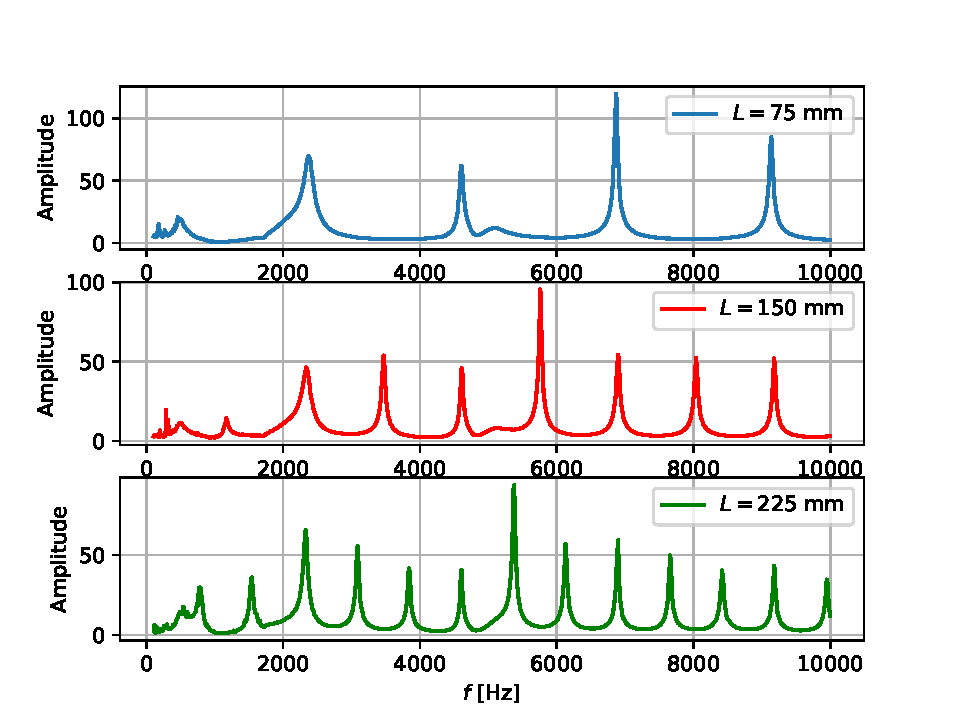
\includegraphics[scale=0.45]{Messwerte/plot1.pdf}
  \caption{Schallamplitude in verschieden langen Röhren $L$ bei variierender Frequenz.}
  \label{fig:plot1}
\end{figure}
\begin{figure}
  \centering
  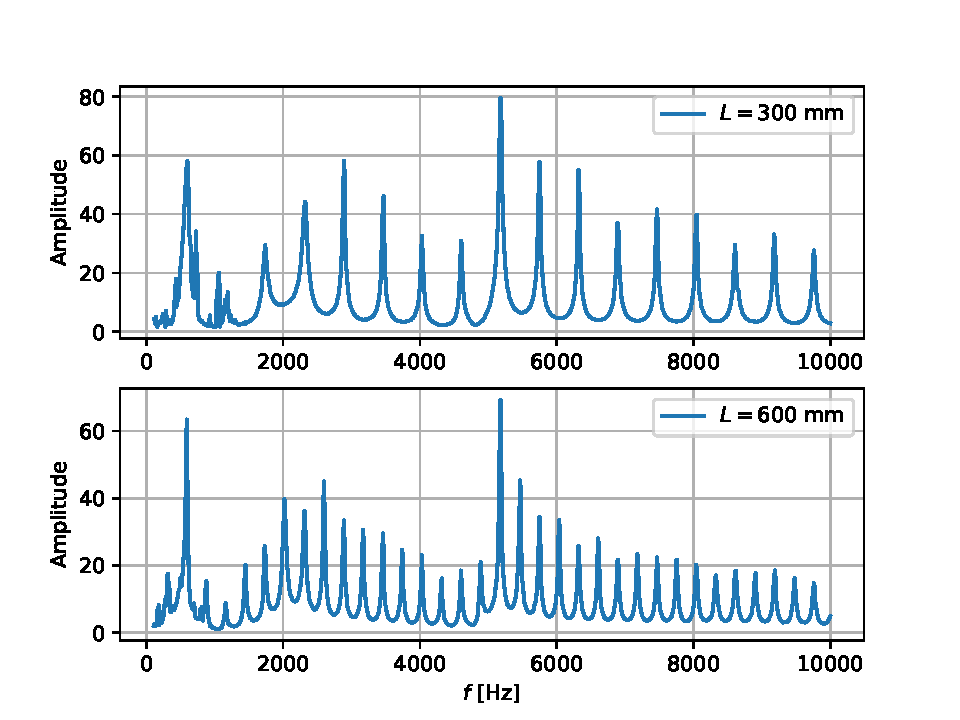
\includegraphics[scale=0.45]{Messwerte/plot2.pdf}
  \caption{Schallamplitude in verschieden langen Röhren $L$ bei variierender Frequenz.}
  \label{fig:plot2}
\end{figure}
Resonanzen treten auf, wenn die Bedingung
\begin{equation}
  2\cdot L=\frac{n\cdot c}{f}
\end{equation}
erfüllt ist. Dabei ist $L$ die Länge der Röhre, $n$ eine Natürliche Zahl, $c$ die Schallgeschwindigkeit und $f$ die Frequenz.
Umgestellt nach $f$:
\begin{equation}
  \underbrace{f}_{y}=\underbrace{\frac{c}{2\cdot L}}_{m}\underbrace{\cdot n}_{x}+\underbrace{0}_{b}.
\end{equation}
Die Steigung $m$ der Linearen Regression entspricht somit $\frac{c}{2\cdot L}$. Aufgelöst nach $c$ ergibt sich damit:
\begin{equation}
  c=m\cdot2\cdot L.
\end{equation}
Da $m$ fehlerbehaftet ist, muss der Ausdruck nach $m$ abgeleitet werden:
\begin{equation}
  \frac{\partial c}{\partial m}=2\cdot L.
\end{equation}
\begin{figure}
  \centering
  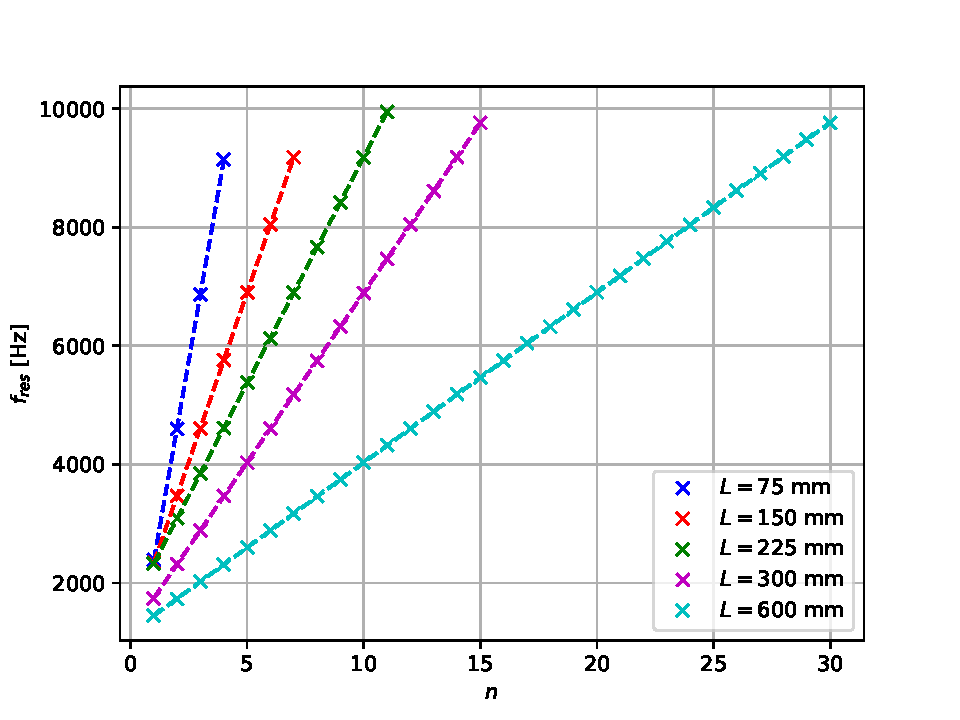
\includegraphics[scale=0.45]{Messwerte/plot3.pdf}
  \caption{Resonanzfrequenzen für Schallwellen bei verschieden Langen Röhren $L$ sowie die entsprechende Lineare Regression.}
  \label{fig:plot3}
\end{figure}
Eingesetzt in die Fehlerentwicklung nach Gauß:
\begin{align}
  \increment c &= \sqrt{\sum_i (\frac{\partial c}{\partial x_i}\cdot\increment x_i)^2}\\
  \increment c &= 2\cdot L\cdot\increment m
\end{align}
Die Steigungen der Linearen Regression $m$, sowie die daraus bestimmte Schallgeschwindigkeit $c$
der verschiedenen Längen $L$ sind in Tabelle \ref{tab:tab1} zu finden.
\begin{table}
  \centering
  \caption{Steigung der Linearen Regression $m$ der Resonanzfrequenzen aufgetragen gegen
  den Index $n$ bei verschiedenen Längen $L$, sowie die daraus berechnete Schallgeschwindigkeit $c$.}
  \label{tab:tab1}
  \begin{tabular}{c|c|c|c|c}
    $L \:/\: \si{\milli\meter}$ & $m \:/\: \si{\hertz}$ & $\increment m \:/\: \si{\hertz}$ & $c \:/\: \si{\meter\per\second}$ & $\increment c \:/\: \si{\meter\per\second}$ \\
    \midrule
    75 & 2252.0 & 10.39 & 337.80 & 1.60 \\
    150 & 1141.1 & 0.89 & 342.32 & 0.27 \\
    225 & 762.0 & 0.48 & 342.90 & 0.22 \\
    300 & 572.4 & 0.30 & 343.41 & 0.18 \\
    600 & 286.7 & 0.07 & 344.06 & 0.09
  \end{tabular}
\end{table}
Der gemittelte Wert für die Schallgeschwindigkeit, welcher sich nach
\begin{equation}
  \overline{x}=\frac{1}{N}\cdot\sum_{i=1}^{N}x_i
\end{equation}
bestimmt, beträgt $c=(342.098\pm 2.22)\si{\meter\per\second}$. Der angegebene Fehler ist
die Standardabweichung, welche nach
\begin{equation}
  \sigma = \overline{x^2}-\overline{x}^2
\end{equation}
bestimmt wurde. Verglichen mit dem Literaturwert von $\SI{343}{\meter\per\second}$
ergibt sich eine Abweichung von  %http://hyperphysics.phy-astr.gsu.edu/hbase/Tables/Soundv.html
\begin{align}
  p =& (\frac{c_{\text{Exp}}}{c_{\text{Lit}}}-1)\cdot100\\
  p =& -0.26\%.
\end{align}
Für $12$ $\SI{50}{\milli\meter}$ ist das Spektrum in Abbildung \ref{fig:plot4} abgebildet. Die Frequenz
ist in Abbildung \ref{fig:plot5} gegen die Wellenzahl $k$ aufgetragen.
\begin{figure}
  \centering
  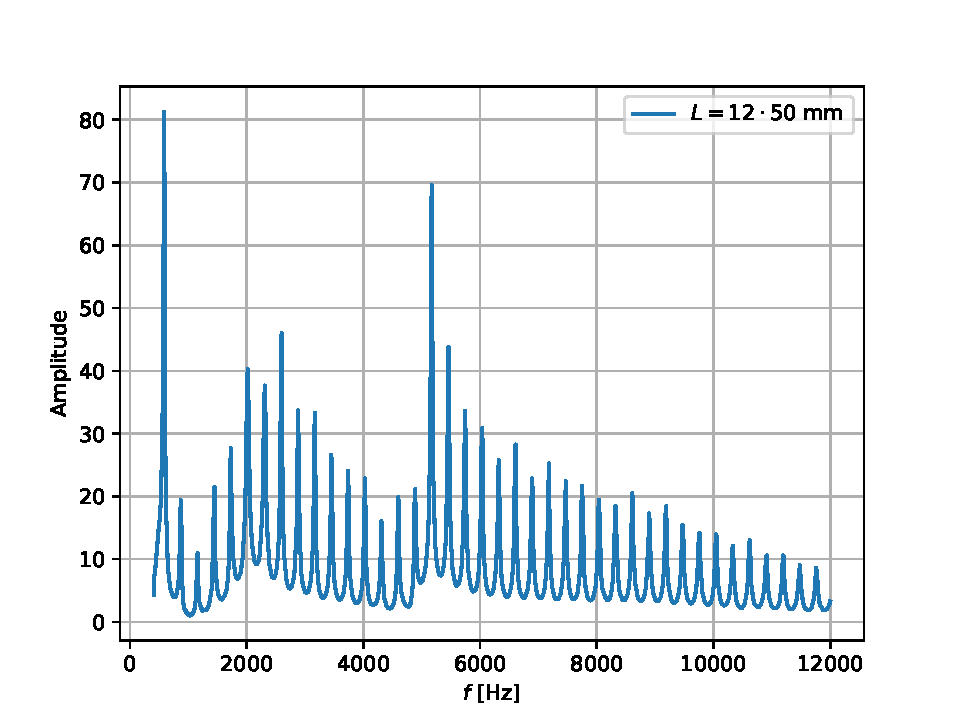
\includegraphics[scale=0.45]{Messwerte/plot4.pdf}
  \caption{Spektrum von einer Röhre, bestehend aus $12$ $\SI{50}{\milli\meter}$ langen Partien.}
  \label{fig:plot4}
\end{figure}
\begin{figure}
  \centering
  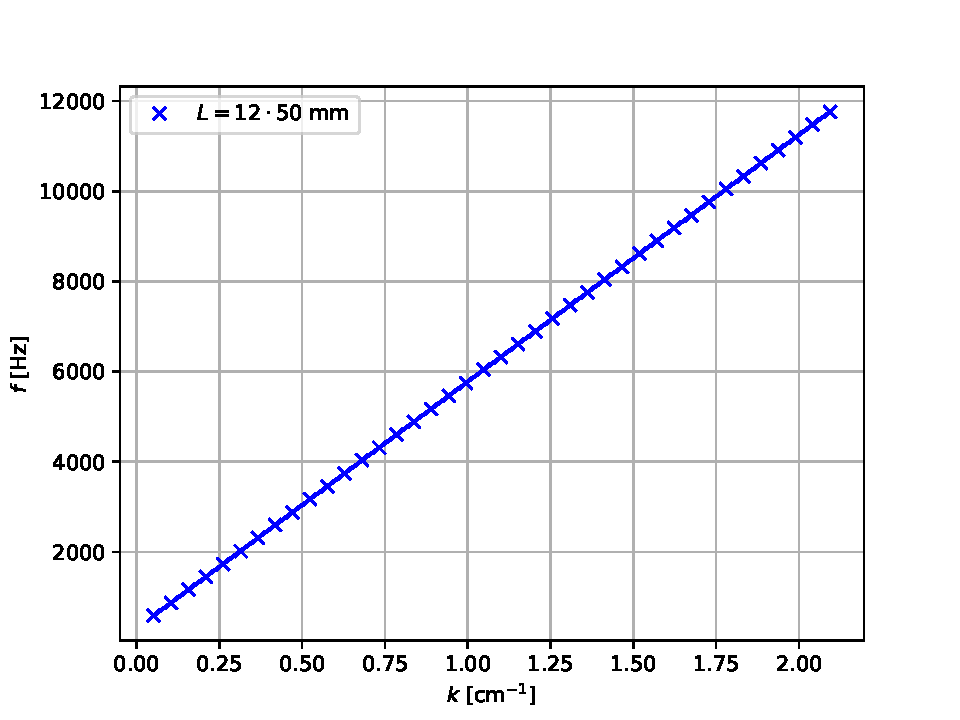
\includegraphics[scale=0.45]{Messwerte/plot5.pdf}
  \caption{Frequenzspektrum aufgetragen gegen die Wellenzahl $k$ für $12$ $\SI{50}{\milli\meter}$ Röhren.}
  \label{fig:plot5}
\end{figure}
Die Wellenzahl $k$ wird mit
\begin{equation}
  k=\frac{2\cdot\pi\cdot n}{L}
\end{equation}
bestimmt. Es wird an der Abbildung deutlich, dass es ein lineares Verhältnis $f(k)=d\cdot k$ sichtbar. Der Fitparameter für die Dispersion beträgt $d=5473.63$.
Somit ist die Dispersionsrelation $f(k)=5473.63\cdot k$. Die Dispersionsrelation der Röhre ohne Streuzentren ist also linear und deckt das Frequenzspektrum mit
äquidistanten Zuständen ab. Die Zustandsdichte ist also konstant und echt größer Null.
\begin{figure}
  \centering
  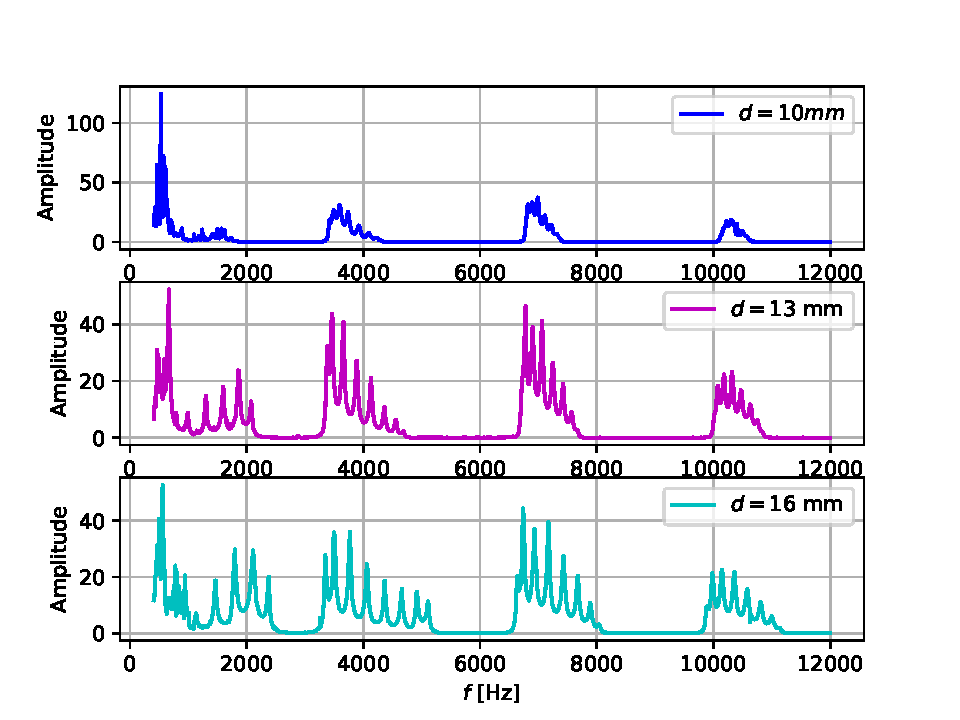
\includegraphics[scale=0.5]{Messwerte/plot6.pdf}
  \caption{Spektrum einer Röhre mit variierendem Durchmesser der Iris zwischen den Rohrabschnitten.}
  \label{fig:plot6}
\end{figure}
\begin{figure}
  \centering
  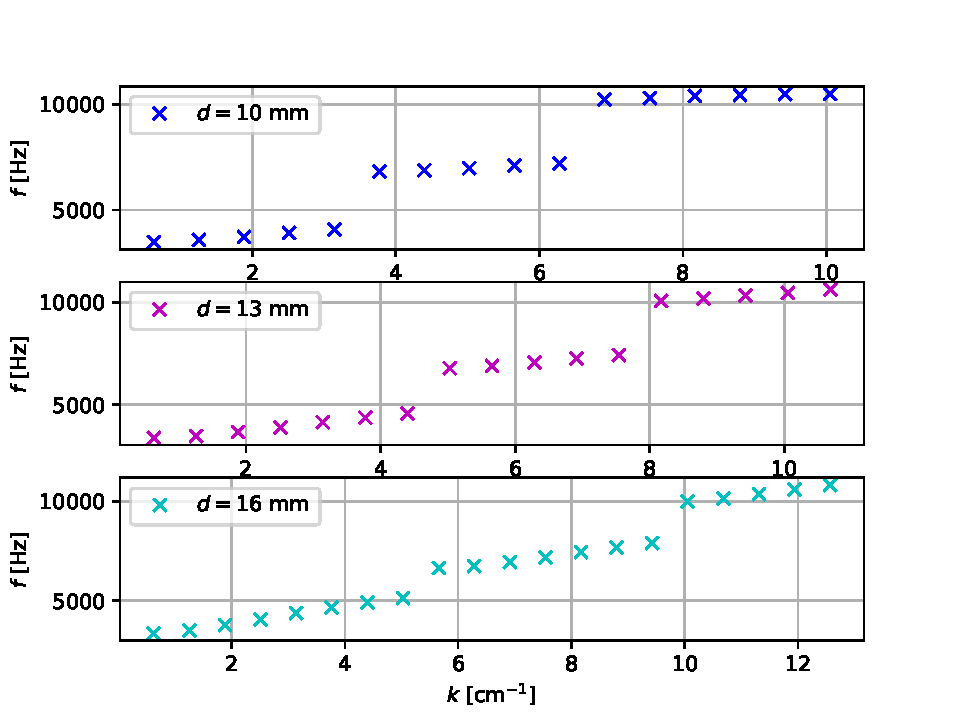
\includegraphics[scale=0.5]{Messwerte/plot7.pdf}
  \caption{Frequenz einer Röhre mit variierendem Durchmesser der Iris zwischen den Rohrabschnitten abhängig von der Wellenzahl $k$.}
  \label{fig:plot7}
\end{figure}
Aus Abbildung \ref{fig:plot7} wird deutlich, dass die Bänder mit steigendem Irisdurchmesser $d$ auch breiter werden.
\begin{figure}
  \centering
  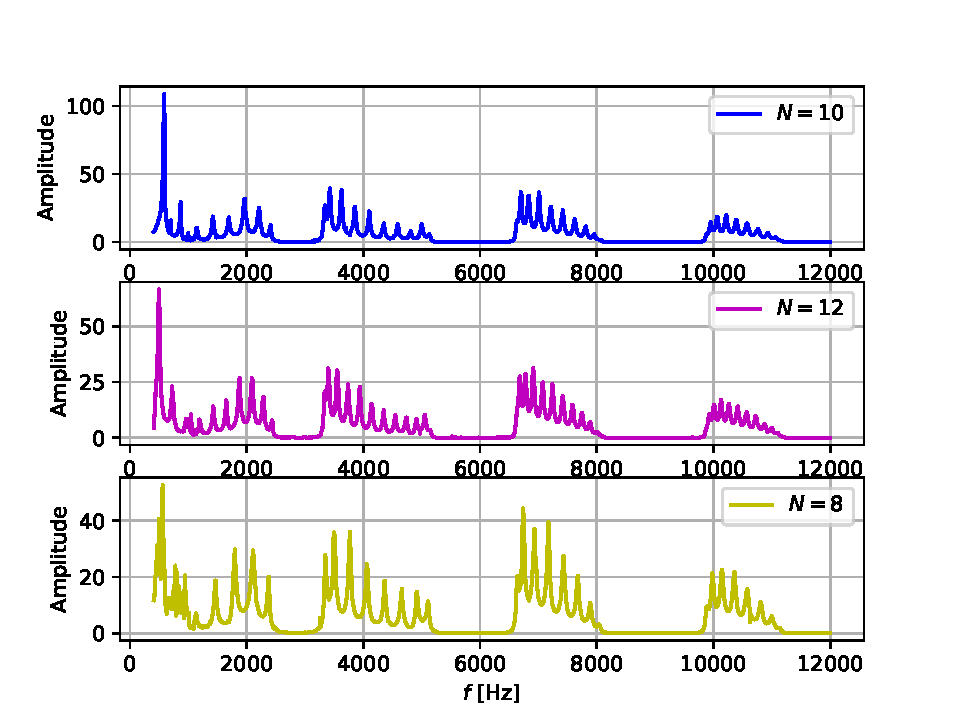
\includegraphics[scale=0.5]{Messwerte/plot8.pdf}
  \caption{Spektren von $n\cdot\SI{50}{\milli\meter}$ Röhren und einem Irisdurchmesser von $d=\SI{16}{\milli\meter}$.}
  \label{fig:plot8}
\end{figure}
Der Vergleich zwischen verschieden Langen Röhren mit einem Irisdurchmesser von $\SI{16}{\milli\meter}$ ist in Abbildung \ref{fig:plot8} zu sehen.
Die Amplitude wird für kleinere Rohrlängen größer, die Resonanzen scheinen bei gleicher Frequenz zu liegen.
\begin{figure}
  \centering
  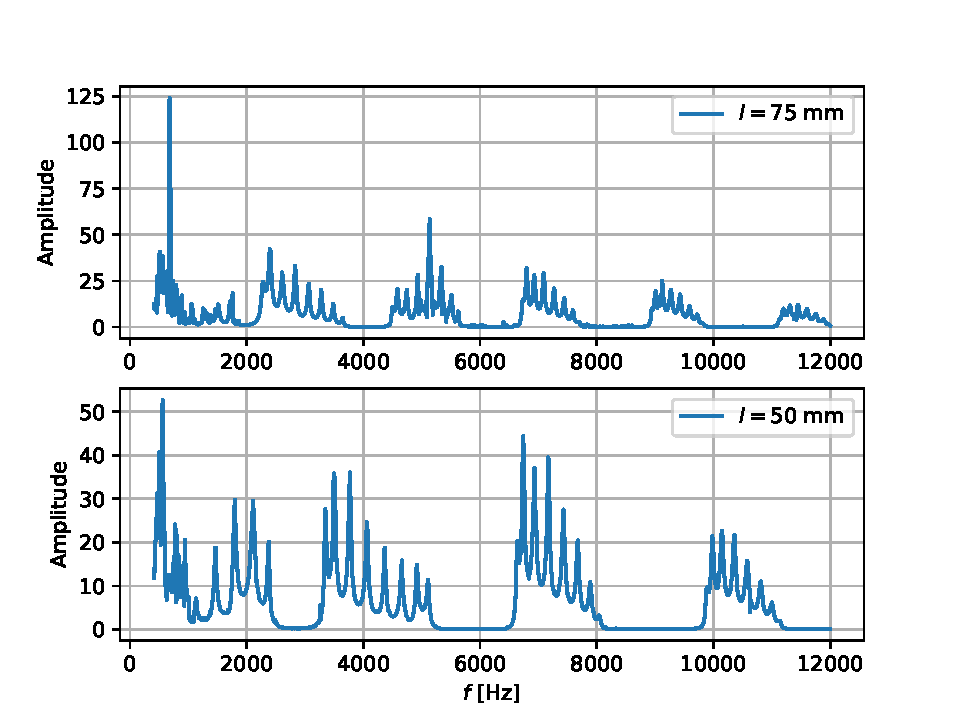
\includegraphics[scale=0.5]{Messwerte/plot9.pdf}
  \caption{Spektren von Röhren, bestehend aus $8$ Stücken mit der Länge $l$ und dem Irisdurchmesser $d=\SI{16}{\milli\meter}$.}
  \label{fig:plot9}
\end{figure}
Beim Vergleich der Spektren für $8$ einzelröhren mit der Länge $l=\SI{50}{\milli\meter}$ und $\SI{75}{\milli\meter}$ (Abbildung \ref{fig:plot9}) fällt auf, dass die
Amplitude bei kleineren Rohrlängen zunimmt und die Resonanzfrequenzen sich verschieben.
\subsection{Näherungen für Molekül-/Atomketten}
Der Vergleich der Spektren einer $\SI{50}{\milli\meter}$ Röhre mit einer $\SI{75}{\milli\meter}$ Röhre (Abbildungen \ref{fig:plot10}) zeigt, dass sich die Anzahl der Resonanzen erhöht und
diese ebenfalls leicht verschoben sind für das längere Rohr.
\begin{figure}
  \centering
  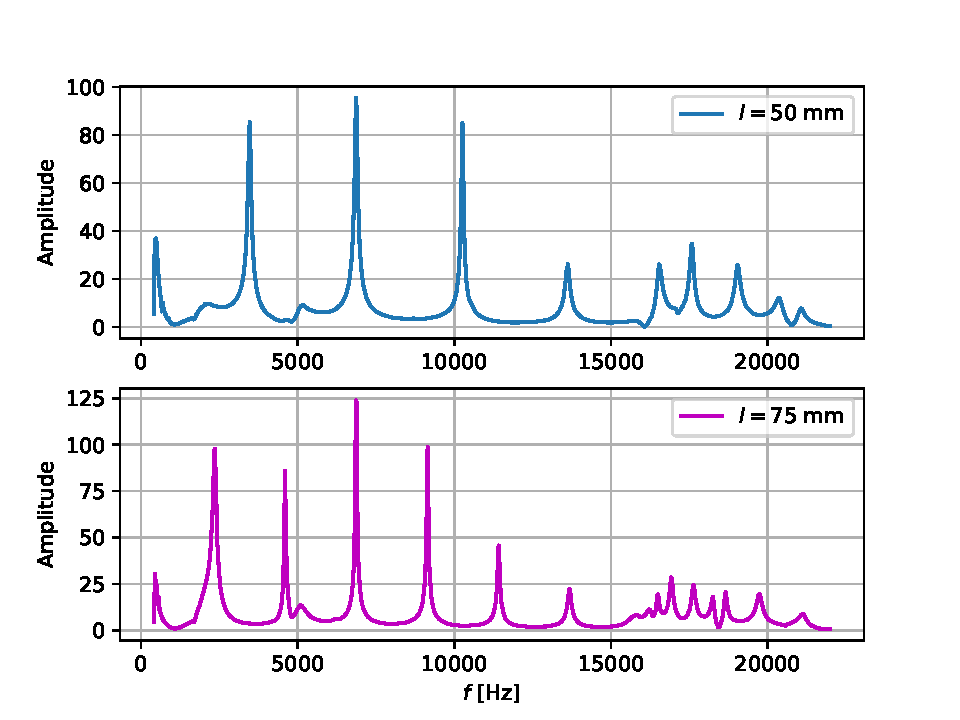
\includegraphics[scale=0.5]{Messwerte/plot10.pdf}
  \caption{Spektren von einer $\SI{50}{\milli\meter}$ und $\SI{75}{\milli\meter}$ Röhre.}
  \label{fig:plot10}
\end{figure}
\begin{figure}
  \centering
  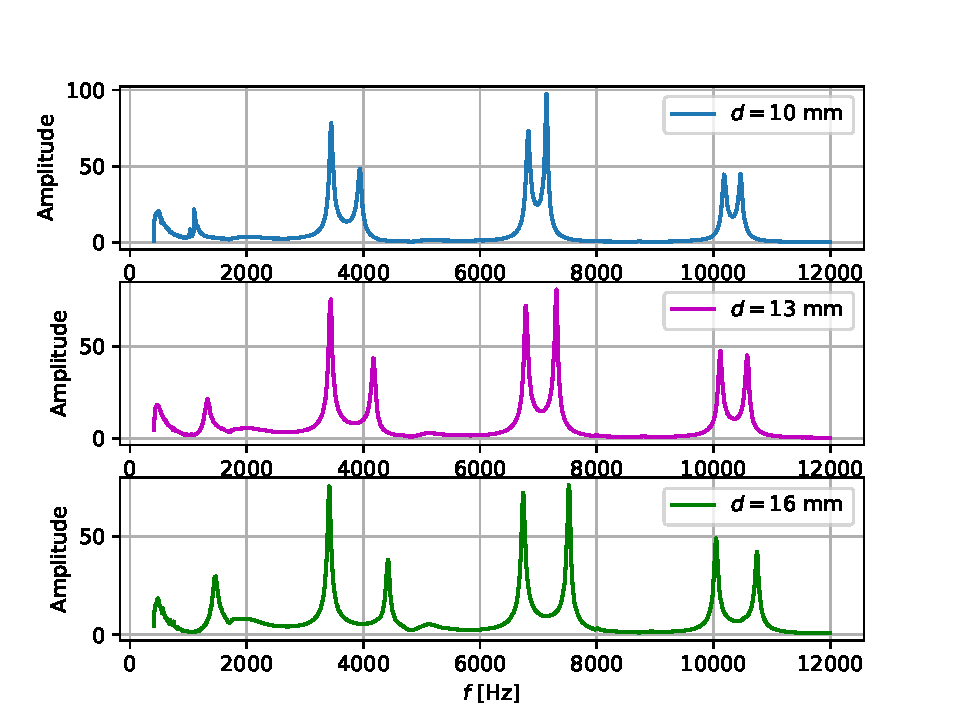
\includegraphics[scale=0.5]{Messwerte/plot11.pdf}
  \caption{Spektren von 2 $\SI{50}{\milli\meter}$ Röhren mit variierenden Irisdurchmesser $d$.}
  \label{fig:plot11}
\end{figure}
Aus Abbildung \ref{fig:plot11} wird ersichtlich, dass mit größerem Irisdurchmesser der Abstand zwischen den Resonanzen steigt. Die Kompression der Bändern
führt zu einer Verringerung der Steigung der einzelnen Dispersionszweige. Da die Frequenz der ersten Resonanz eines Bandes unverändert bleibt,
führt dieser Effekt zu einer Vergrößerung der Bandlücke.
\begin{figure}
  \centering
  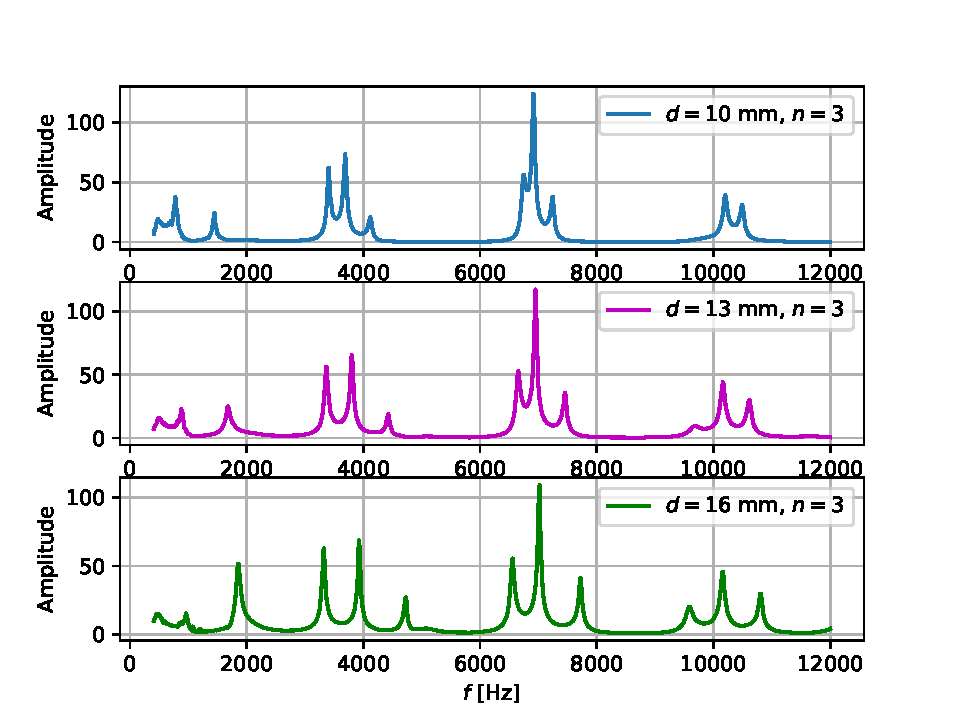
\includegraphics[scale=0.5]{Messwerte/plot12.pdf}
  \caption{Spektren von $n$ Elementarzellen mit variierendem Irisdurchmesser $d$.}
  \label{fig:plot12}
\end{figure}
\begin{figure}
  \centering
  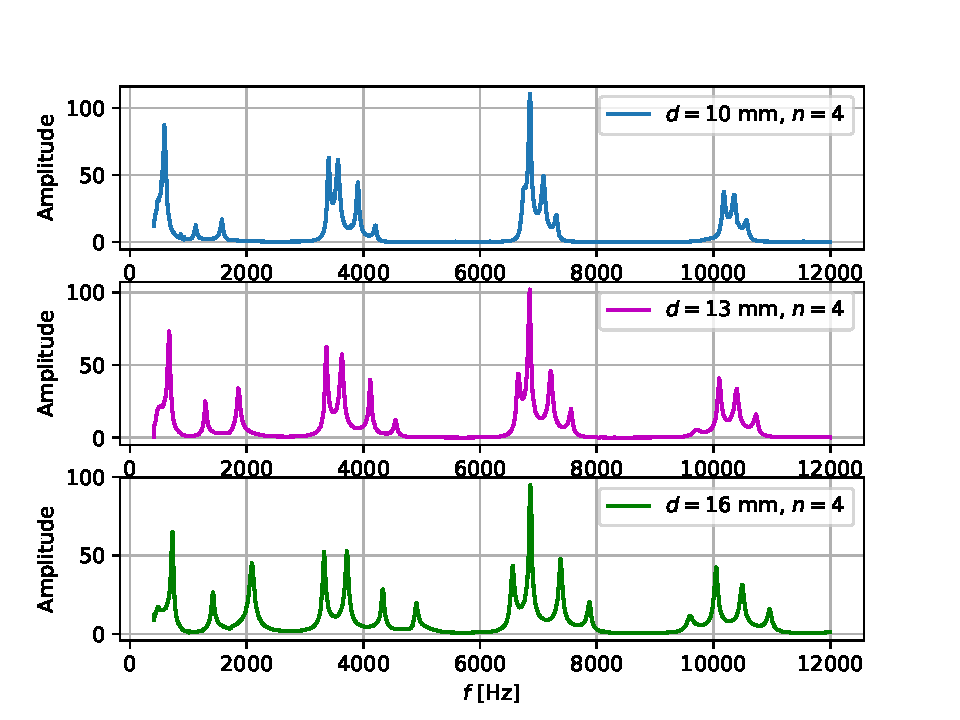
\includegraphics[scale=0.5]{Messwerte/plot13.pdf}
  \caption{Spektren von $n$ Elementarzellen mit variierendem Irisdurchmesser $d$.}
  \label{fig:plot13}
\end{figure}
\begin{figure}
  \centering
  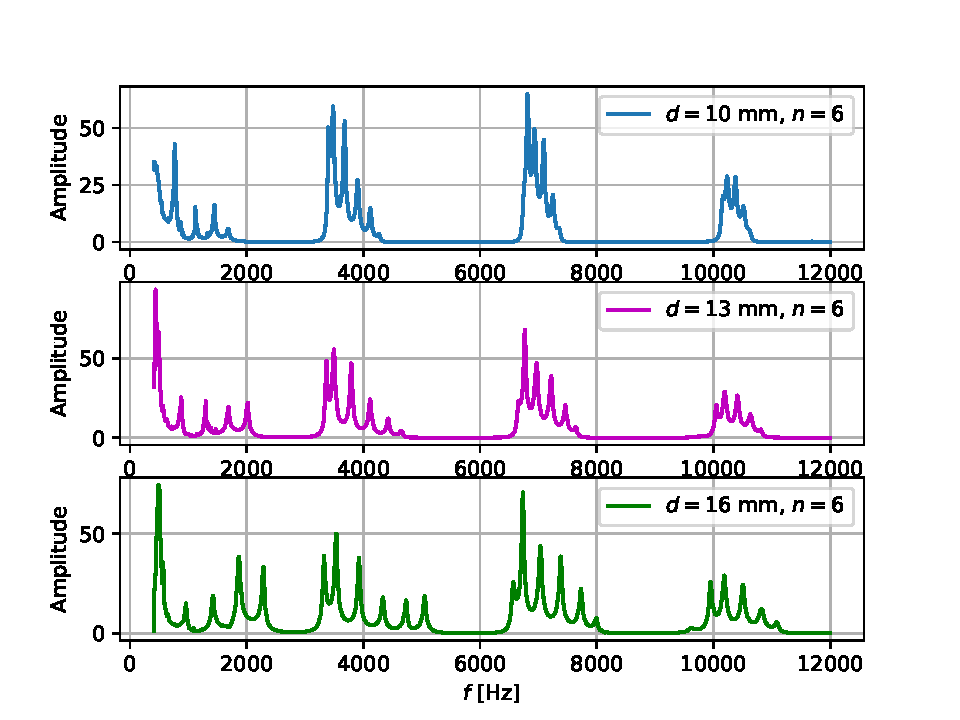
\includegraphics[scale=0.5]{Messwerte/plot14.pdf}
  \caption{Spektren von $n$ Elementarzellen mit variierendem Irisdurchmesser $d$.}
  \label{fig:plot14}
\end{figure}
\begin{figure}
  \centering
  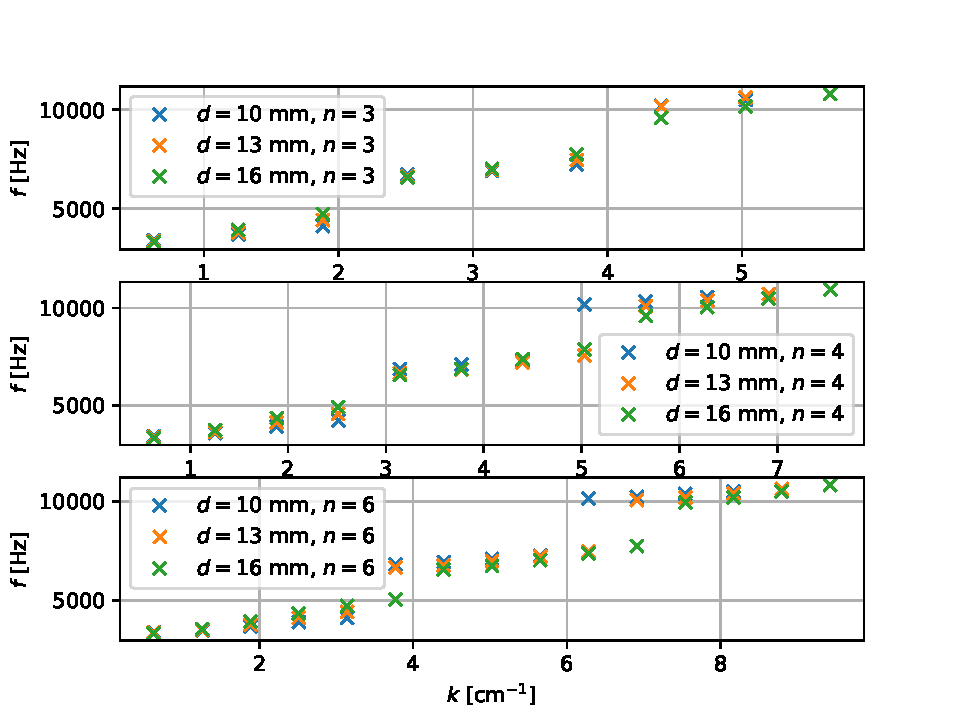
\includegraphics[scale=0.5]{Messwerte/plot15.pdf}
  \caption{Bandstrukturen von $n$ Elementarzellen mit variierendem Irisdurchmesser $d$.}
  \label{fig:plot15}
\end{figure}
Aus Abbildung \ref{fig:plot15} wird deutlich, dass sich die Bandbreiten mit zunehmender Anzahl an Elementarzellen erhöht, sonst bleiben die Bandstrukuren jedoch gleich.
Während die ersten beiden Bänder stark gestört sind, zeigen die Bänder mit höherer Elementarzellenzahl eindrucksvoll, wie sich die Bandstruktur sukzessive beim
Hinzufügen von Elementarzellen aufbaut.
\begin{figure}
  \centering
  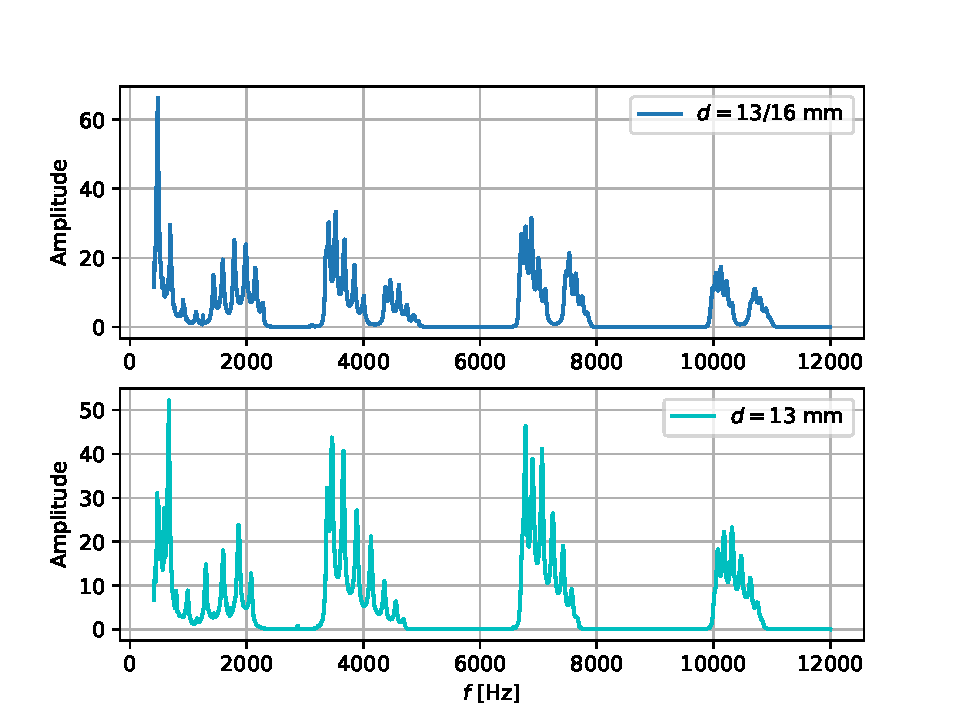
\includegraphics[scale=0.5]{Messwerte/plot16.pdf}
  \caption{Spektrum mit $12$ $\SI{50}{\milli\meter}$ Röhren mit alternierenden Irisdurchmesser von $13$ und $\SI{16}{\milli\meter}$. Zum Vergleich
  das Spektrum von $12$ $\SI{50}{\milli\meter}$ Röhren mit einem festen Irisdurchmesser von $\SI{13}{\milli\meter}$.}
  \label{fig:plot16}
\end{figure}
Die Resonanzen aus den beiden Grafiken aus Abbildung \ref{fig:plot16} scheinen gleich zu sein, jediglich bei den alternierenden Irisdurchmesser spalten sich die
Resonanzen auf.
\begin{figure}
  \centering
  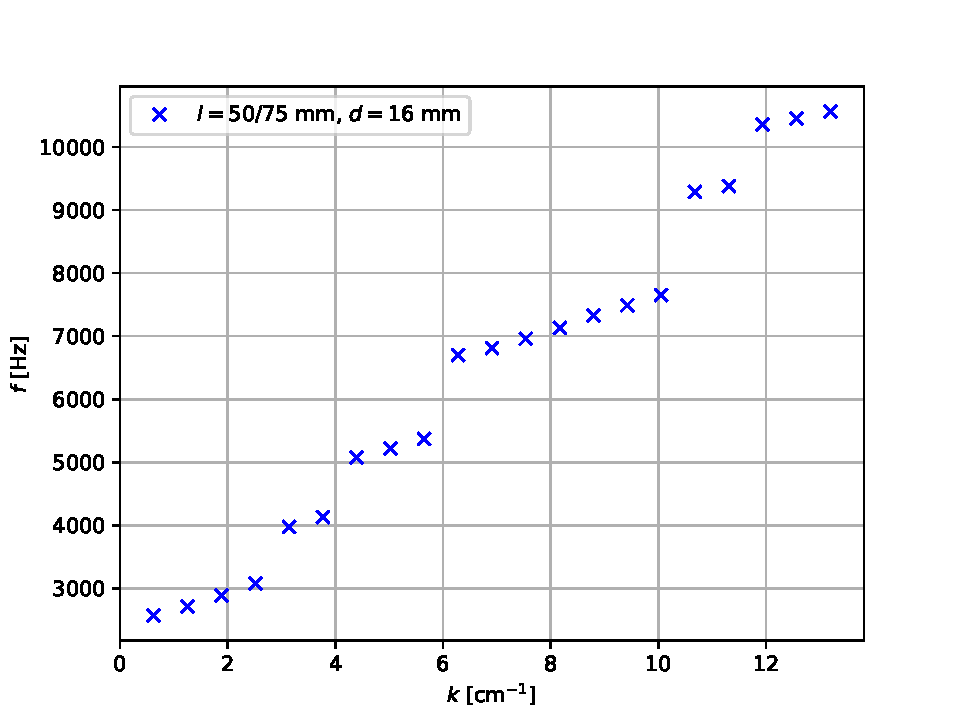
\includegraphics[scale=0.5]{Messwerte/plot17.pdf}
  \caption{Bandstruktur von $5$ Elementarzellen, welche aus $\SI{50}{\milli\meter}$ und $\SI{75}{\milli\meter}$ Röhren
  und $\SI{16}{\milli\meter}$ Irisdurchmesser bestehen.}
  \label{fig:plot17}
\end{figure}

\begin{figure}
  \centering
  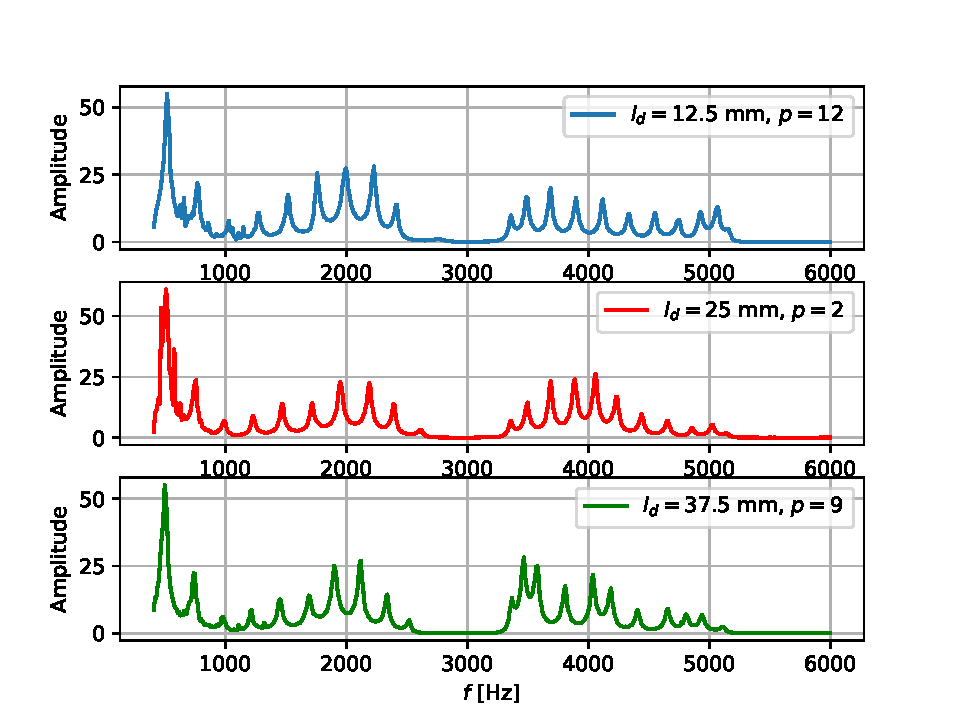
\includegraphics[scale=0.5]{Messwerte/plot18.pdf}
  \caption{Spektrum von $12$ $\SI{50}{\milli\meter}$ Röhren mit einem Irisdurchmesser von $\SI{16}{\milli\meter}$. Dazu wurde ein Defekt an der Stelle $p$ eingebaut
  mit der Länge $l_d$.}
  \label{fig:plot18}
\end{figure}
\begin{figure}
  \centering
  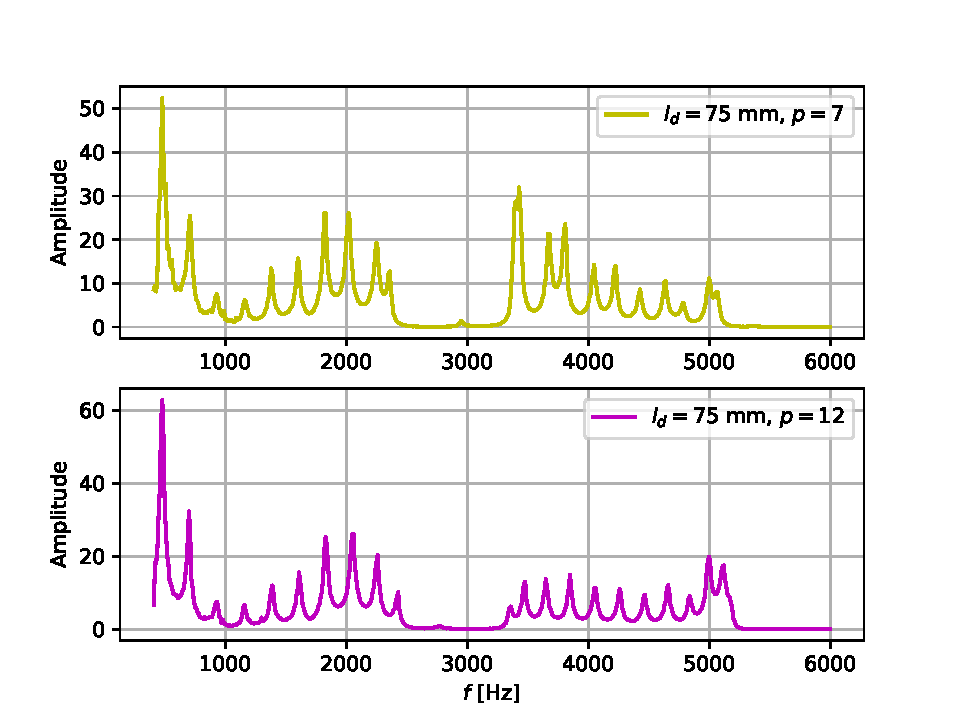
\includegraphics[scale=0.5]{Messwerte/plot19.pdf}
  \caption{Spektrum von $12$ $\SI{50}{\milli\meter}$ Röhren mit einem Irisdurchmesser von $\SI{16}{\milli\meter}$. Dazu wurde ein Defekt an der Stelle $p$ eingebaut
  mit der Länge $l_d$.}
  \label{fig:plot19}
\end{figure}
Aus Abbildung \ref{fig:plot18} und \ref{fig:plot19} wird deutlich, dass durch den Einbau des Defekts sich in der ersten Bandlücke ein neuer Zustand ausbildet.
Durch Verschiebung des Defektes nach innen, verschiebt sich auch die Position des Defektmode weiter nach rechts, konvergiert jedoch gegen die mittige Störung und wandert
dann wieder nach links, wenn der Defekt über die Mitte hinausgeschoben wird.Das Analogon in der Festkorperphysik ist das Dotieren eines Einkristalls, wie es z.B. in der
Halbleiterelektronik üblich ist. Donatoren erzeugen dabei Zustände innerhalb der Bandlücke nahe am Leitungsband während Akzeptoren nahe am Valenzband
(also an der Unterkanteeiner Lücke) neue Zustände einfügen.
